
%(BEGIN_QUESTION)
% Copyright 2005, Tony R. Kuphaldt, released under the Creative Commons Attribution License (v 1.0)
% This means you may do almost anything with this work of mine, so long as you give me proper credit

Kalkulus er en gren av matematikken som oppsto fra vitenskapelige spørsmål om {\it endringsrater}. De enkleste endringsratene for de fleste å forstå er de som handler om tid. For eksempel vil en student som ser sparekontoen sin krympe over tid mens hen betaler skolepenger og andre utgifter være svært opptatt av endringsrater ({\it kroner per dag} som brukes).

Endringsrater uttrykkes symbolsk i matematiske ligninger med ``derivert''-notasjon. For eksempel: hvis variabelen $S$ representerer beløpet på studentens sparekonto og $t$ representerer tid, vil endringsraten for penger over tid (den {\it tidsderiverte} av kontosaldoen) skrives som $dS \over dt$. Prosessen med å beregne denne endringsraten fra en registrering av kontosaldo over tid, eller fra en ligning som beskriver saldoen over tid, kalles {\it derivasjon}.

\vskip 10pt

Anta at student {\bf A} har konto i Humongous Savings and Loan der daglige kontosaldoer dokumenteres for kundene, mens student {\bf B} har konto i Isaac Newton Credit Union der kontoutskriften kun viser rater for {\it endring} i kontosaldo. Disse endringsratene oppgis alltid i enheten dollar per dag, beregnet ved slutten av hver dag. Hvis begge studentene startet med nøyaktig samme beløp, og tok ut nøyaktig samme beløp til samme tidspunkter, vil de to utskriftene se slik ut:

$$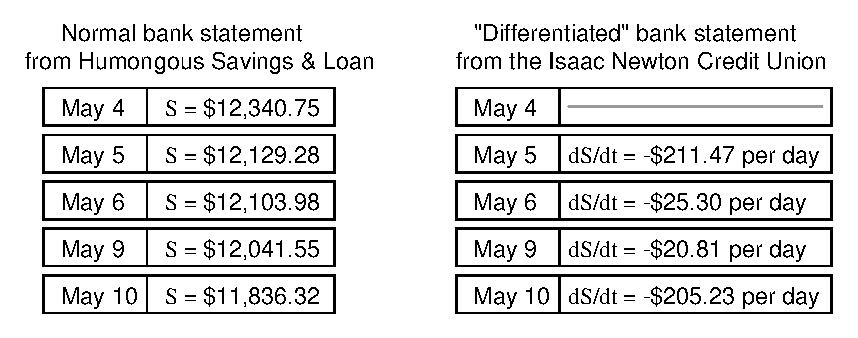
\includegraphics[width=15.5cm]{i01563x01.eps}$$

Forklar hvordan Isaac Newton Credit Union beregner deriverten ($dS \over dt$) fra saldoverdiene (tilsvarende $S$ i utskriften fra Humongous Savings \& Loan), og forklar deretter hvordan studenten som bruker Isaac Newton Credit Union kan finne ut hvor mye penger som står på konto til enhver tid uten slike saldotall.

Hint: prosessen med å beregne en variabelverdi fra endringsrater kalles {\it integrasjon} i kalkulus. Det er den motsatte (inverse) funksjonen av derivasjon.

\underbar{file i01563}
%(END_QUESTION)





%(BEGIN_ANSWER)

Isaac Newton Credit Union deriverer $S$ ved å dele differansen mellom påfølgende saldoer på antall dager mellom disse saldoverdiene. Derivasjon er grunnleggende en divisjonsprosess.

For å integrere $dS\over dt$-verdiene i Credit Union-utskriften slik at vi får verdier for $S$, må vi enten legge til eller trekke fra daglige endringsrater gjentatte ganger, med utgangspunkt i en startsaldo. Integrasjon er derfor grunnleggende en multiplikasjonsprosess.

\vskip 10pt

Oppfølgingsspørsmål: forklar hvorfor en startsaldo er helt nødvendig for at studenten i Isaac Newton Credit Union skal kunne bestemme kontosaldoen til et hvilket som helst tidspunkt. Hvorfor ville det være umulig å finne hvor mye penger kontoen inneholder hvis den eneste informasjonen var $dS \over dt$-verdiene?

%(END_ANSWER)





%(BEGIN_NOTES)

Hensikten med denne oppgaven er å introdusere integralbegrepet på en måte studentene kjenner igjen. Forhåpentligvis er startsituasjonen med en krympende sparekonto noe de kan relatere seg til.

Noen studenter kan spørre hvorfor differensialnotasjonen $dS \over dt$ brukes i stedet for differansenotasjonen $\Delta S \over \Delta t$ i dette eksemplet, siden endringsratene alltid beregnes ved subtraksjon av to datapunkter (som dermed antyder $\Delta$). Siden funksjonen her er stykkevis og ikke kontinuerlig, kan man argumentere for at den ikke er deriverbar i de relevante punktene. Min hensikt med differensialnotasjon er å gjøre studentene kjent med derivertbegrepet i en sammenheng de lett forstår, selv om detaljene i anvendelsen kunne tilsi en annen notasjon.

Før du tenker på å korrigere $dS \over dt$-tallet for 9. mai, fra \$20.81 per day til \$62.43 per day, merk at dette er en {\it per dag}-rate, og at det er tre dager mellom 9. mai og forrige saldooppføring!

%INDEX% Mathematics, calculus: integral and derivative related to finances

%(END_NOTES)

